g% !TeX root = ../my-thesis.tex
\chapter{Beispiel zur Nutzung}
\section{Abkürzungen und Zitate}
Jedes Acronym hat einen Identifier, der komplett klein geschrieben wird. Im Beispiel: volte~-~nicht zu verwechseln mit der Abkürzung selbst (hier VoLTE). Im Abkürzungsverzeichnis werden alle Abkürzungen aufgelistet, mit allen Stellen, an denen sie Dokument verwendet wurden. 

\begin{minipage}{.6\textwidth}
\begin{lstlisting}[language=latex]
\ac{volte} % Erste Verwendung: 
% Langform (Abkürzung)
\ac{volte} % Zweite Verwendung: Abkürzung
\acs{isdn} % s = short: Abkürzung
\acl{ims} % l = long: Langform
\acf{iad} % f = full: Langform (Kurzform)
\end{lstlisting}   
\end{minipage}
\begin{minipage}{.4\textwidth}
	\footnotesize
	\textbf{Ergibt:}\\
	\ac{volte}\\
	\ac{volte}\\
	\acs{isdn}\\
	\acl{ims}\\
	\acf{iad} 
\end{minipage}

Bei der ersten Verwendung, wird die Langform ausgegeben, alle weitere Nutzungen der Abkürzung ergeben nur die Kurzform. Somit muss man nicht überlegen, ob die Abkürzung schon mal verwendet wurde, wie folgender Satz zeigt: 

\Ac{volte} ist eine tolle Erfindung \cite{3GPP.TS.24.228.v5.15.0}. Die Signalisierung läuft über das \ac{sip}~\cite{wikiNik}. \cite[S.~23]{fernandezgallardo_InstitutFurSoftwaretechnik_2017}
\cite[S.~50]{arnold2000java}

Auch das Zitieren von Quellen ist mit \LaTeX{} ein Kinderspiel! Treffe ich eine Aussage, so muss ich sie belegen~\cite{rfc2693}. Dies geschieht mit dem Befehl \lstinline[language=latex]|\cite{<bibid>}|. Mehrere Quellen werden durch eine kommagetrennte Liste an \texttt{BibIDs} im \texttt{cite} Befehl zitiert: \lstinline[language=latex]|\cite{<bibid1>, <bibid2>, <bibid2>}| ergibt: schrägstrich cite{rfc1, rfc1754, rfc1971}. Alle zitierten Quellen landen im Literaturverzeichnis.
\section{Bilder und Verweise}
\begin{figure}[ht]
	\centering
	\includegraphics[width=.85\linewidth]{turn-channeldata}
	\caption{Ein Vektografik Screenshot}
	\label{fig:turn-channeldata}
\end{figure}

Falls möglich sollten stets Vektorgrafiken verwendet werden. Diese können zum Beispiel mit Visio erstellt und als PDF exportiert werden. Die PDF Datei kann dann in \LaTeX{} als Grafik verwendet werden. Der Code hierfür lautet wie folgt:

% the float option prevents figures to be placed in the listing but also prevents the listing from spanning multiple pages
\begin{lstlisting}[language=latex,float]
\begin{figure}
	\centering %Zentrieren
	\includegraphics[width=.85\linewidth]{turn-channeldata} % Grafik einbinden (ohne Dateiendung) und auf 85 % der Seitenbreite Skalieren
	\caption{Ein Vektografik Screenshot} % Die Bildunterschrift
	\label{fig:turn-channeldata} % Das Label, mit dem die Grafik im Text referenziert werden kann
\end{figure}
\end{lstlisting}

Im Text kann ich auf eingebundene Abbildungen verweisen. In \autoref{fig:turn-channeldata} ist ein Vektorgrafik Screenshot zu sehen. Verwendet man \verb|\autoref{<label>}|, wird die Bezeichnung (Abbildung, Tabelle, Abschnitt\dots) automatisch ergänzt.


\begin{figure}[ht]
	\newcounter{density}
	\setcounter{density}{20}
	\centering
	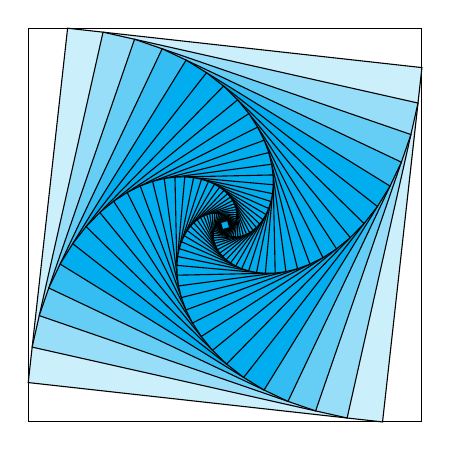
\begin{tikzpicture}
	\def\couleur{cyan}
	\path[coordinate] (0,0)  coordinate(A)
	++( 90:5cm) coordinate(B)
	++(0:5cm) coordinate(C)
	++(-90:5cm) coordinate(D);
	\draw[fill=\couleur!\thedensity] (A) -- (B) -- (C) --(D) -- cycle;
	\foreach \x in {1,...,40}{%
		\pgfmathsetcounter{density}{\thedensity+20}
		\setcounter{density}{\thedensity}
		\path[coordinate] coordinate(X) at (A){};
		\path[coordinate] (A) -- (B) coordinate[pos=.10](A)
		-- (C) coordinate[pos=.10](B)
		-- (D) coordinate[pos=.10](C)
		-- (X) coordinate[pos=.10](D);
		\draw[fill=\couleur!\thedensity] (A)--(B)--(C)-- (D) -- cycle;
	}
	\end{tikzpicture}
	\caption{Rotated square from
		\href{http://www.texample.net/tikz/examples/rotated-polygons/}{texample.net}.}
	\label{fig:tikz1}
\end{figure}

Grafiken können auch direkt in \LaTeX{} mittles des TikZ Paketes erstellt werden (\autoref{fig:tikz1}). Auch verschiedenste Diagramme und Plots sind möglich (\autoref{fig:tikz2}). Zur vereinfachten Erstellung sind Tools, wie z.\,B. \href{https://www.mathcha.io}{https://www.mathcha.io} hilfreich.

\begin{figure}[ht]
	
	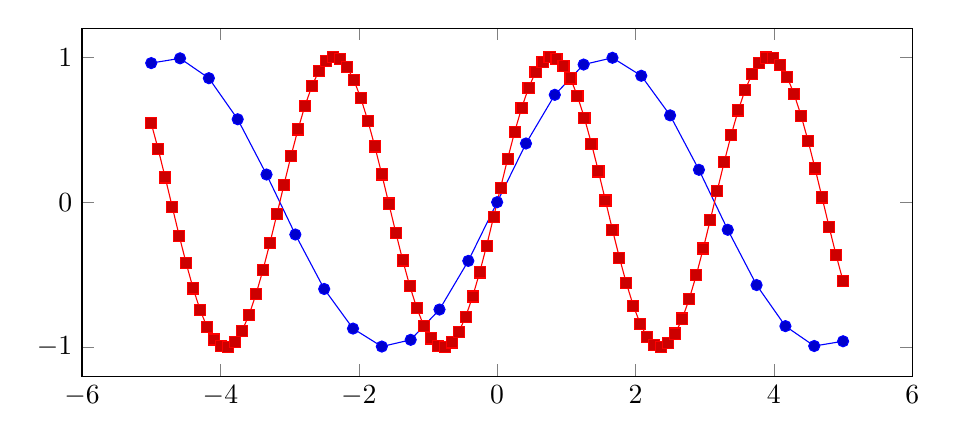
\begin{tikzpicture}
		\begin{axis}[
%		mlineplot,
		width=\textwidth,
		height=6cm,
		]
		
		\addplot {sin(deg(x))};
		\addplot+[samples=100] {sin(deg(2*x))};
		
		\end{axis}
	\end{tikzpicture}
	\caption{Ein Sinusplot mittels TiKZ}
	\label{fig:tikz2}
\end{figure}

\begin{figure}[ht]
	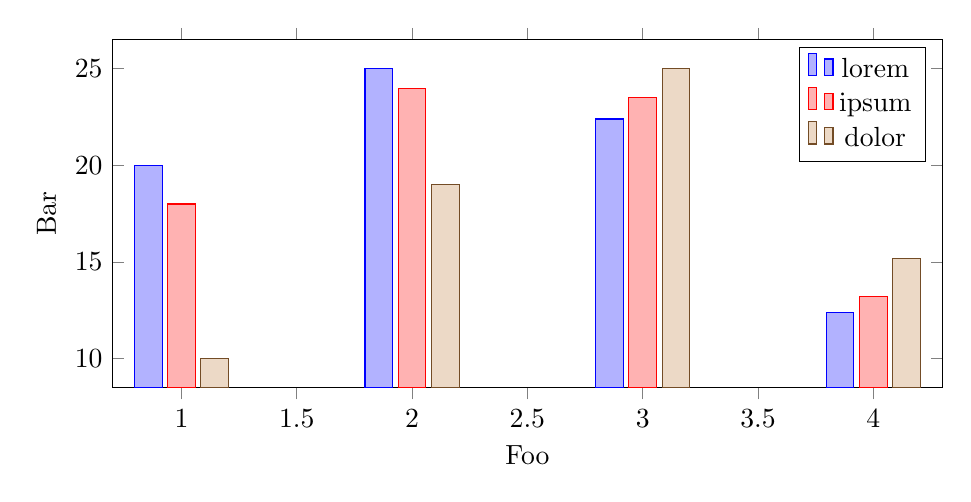
\begin{tikzpicture}
	\begin{axis}[
	ybar,
	xlabel={Foo},
	ylabel={Bar},
	width=\textwidth,
	height=6cm,
	]
	
	\addplot plot coordinates {(1, 20) (2, 25) (3, 22.4) (4, 12.4)};
	\addplot plot coordinates {(1, 18) (2, 24) (3, 23.5) (4, 13.2)};
	\addplot plot coordinates {(1, 10) (2, 19) (3, 25) (4, 15.2)};
	
	\legend{lorem, ipsum, dolor}
	
	\end{axis}
	\end{tikzpicture}
	\caption{Ein Balkendiagramm}
	\label{fig:tikz3}
\end{figure}

Wie in \autoref{fig:tikz3} zu sehen, sind auch Balkendiagramme möglich.

Mit \verb|\autoref{<label>}| kann man auch auf Abschnitte oder Kapitel verweisen. Im PDF wird automatisch eine Verlinkung hinzugefügt (siehe \autoref{sec:kommunikationsvorgange}).

\section{Tabellen}
\begin{otherlanguage*}{USenglish} % Switch document language temporarily but keep labels in main language. For better hyphenation! Use the unstarred variant to translate the labels as well.
\begin{table}
	\centering
	\caption[Modes of operation according to \glsentrytext{itu-t}]{Modes of operation according to \textcite{ITU-T.P.564}}
	\label{tab:modes_P.564}
	\begin{tabularx}{\textwidth}{@{}lclX@{}}
		\toprule
		\multicolumn{1}{c}{\textbf{Class}} & \textbf{Mode} & \multicolumn{1}{c}{\textbf{Name}} & \multicolumn{1}{c}{\textbf{Description}}                                                                            \\ \midrule
		\multirow{5}{*}{Midpoint}          & \multirow{2}{*}{A}             & \multirow{2}{*}{Dynamic operation}                 & The model uses information from RTCP-XR packets to optimize its prediction. \\ \cmidrule{2-4}
		& \multirow{2}{*}{B}             & \multirow{2}{*}{Static operation}                  & The model has been optimized or configured using \textit{a priori} knowledge of the endpoint.                                \\ \midrule
		\multirow{2}{*}{Endpoint}                            & \multirow{2}{*}{C}             & \multirow{2}{*}{Embedded operation}                & The model is co-located with the jitter buffer in the endpoint and has access to the jitter buffer.                 \\ \bottomrule
	\end{tabularx}

\end{table}
\end{otherlanguage*}
Tabellen können kompliziert in der Erstellung sein. Zum Glück gibt es Hilfsmittel wie den \enquote{\LaTeX{} Tables Generator}~\footnote{\href{https://www.tablesgenerator.com/}{https://www.tablesgenerator.com/}}. Dann ist auch die Erstellung von komplexeren Layouts wie in \autoref{tab:modes_P.564} kein Problem.


\section{Quellcode}
Auch Quellcode mit automatischem Syntaxhighlighting kann eingebunden werden. Die Referenzierung funktioniert auch hier (siehe \autoref{lst:signalexample}). Für noch schönere Quellcodelistings empfiehlt sich das Paket \href{https://ctan.org/pkg/minted?lang=de}{\texttt{minted}}, welches anstelle des \texttt{listings} Paket verwendet wird (Python benötigt!).
\begin{lstlisting}[language=c,caption={[Ein einfaches Quellcodelisting]Ein einfaches Quellcodelisting~\cite{wolf_LinuxsystemprogrammierenCKurs_2003}},label=lst:signalexample]
#include <stdio.h>
#include <stdlib.h>
#include <signal.h>

void sigfunc(int sig) {
	char c;
	if(sig != SIGINT)
		return;
	else {
		printf("\nWollen sie das Programm beenden (j/n) : ");
		c=getchar();
		if(c=='j')
			exit(0);
		return;
	}
}
int main() {
	int i;
	signal(SIGINT,sigfunc);
	while(1) {
	printf("Die Endlosschleife können sie mit STRG-C beenden");
	for(i=0;i<48;i++) {
		printf("\b"); //Cursor nach links bewegen
	}
	return 0;
}
\end{lstlisting}

\section{Sonstiges}
Es wird auch eine Umgebung für Beschreibungen bereitgestellt, bei denen das Label rechtsbündig ausgerichtet ist und die Beschreibung linksbündig. In die eckigen Klammern kommt das längste Label, damit \LaTeX{} die Abstände automatisch berechnen kann. Im Folgenden wird ein Beispiel für so eine Umgebung gebracht:

\begin{lstlisting}[language=latex,breaklines]
\begin{aligneddescription}[Registration success rate]
	\item[Registration success rate] describes the rate of successful registration attempts with the \ac{webrtc} signaling server.
	\item[Service availability] is defined in terms of capacity to establish calls from, and to \ac{webrtc} endpoints. 
	\item[Post dialing delay] is the time interval (in seconds) between the end of dialing by the caller and the reception back by him of the appropriate ringing tone or recorded announcement.
	\item[Call drop rate] equals service continuity in terms of capacity to maintain calls to their normal end.
\end{aligneddescription}
\end{lstlisting}
Das Ergebnis sieht wie folgt aus:
\begin{otherlanguage*}{USenglish} % switch to english hyphenation again
\begin{aligneddescription}[Registration success rate]
	\item[Registration success rate] describes the rate of successful registration attempts with the \ac{webrtc} signaling server.
	\item[Service availability] is defined in terms of capacity to establish calls from, and to \ac{webrtc} endpoints. 
	\item[Post dialing delay] is the time interval (in seconds) between the end of dialing by the caller and the reception back by him of the appropriate ringing tone or recorded announcement.
	\item[Call drop rate] equals service continuity in terms of capacity to maintain calls to their normal end.
\end{aligneddescription}
\end{otherlanguage*}

Des Weiteren bietet \KOMAScript{} die \texttt{labeling} Umgebung. Diese arbeitet ähnlich wie die \texttt{aligneddesription} Umgebung, jedoch sind die Labels linksbündig ausgerichtet. Das Ergebnis sieht wie folgt aus:

\begin{otherlanguage*}{USenglish} % switch to english hyphenation again
\begin{labeling}{Registration success rate}
	\item[Registration success rate] describes the rate of successful registration attempts with the \ac{webrtc} signaling server.
	\item[Service availability] is defined in terms of capacity to establish calls from, and to \ac{webrtc} endpoints. 
	\item[Post dialing delay] is the time interval (in seconds) between the end of dialing by the caller and the reception back by him of the appropriate ringing tone or recorded announcement.
	\item[Call drop rate] equals service continuity in terms of capacity to maintain calls to their normal end.
\end{labeling}
\end{otherlanguage*}

Hier zum Vergleich die Standard \texttt{description} Umgebung:

\begin{otherlanguage*}{USenglish} % switch to english hyphenation again
\begin{description}
	\item[Registration success rate] describes the rate of successful registration attempts with the \ac{webrtc} signaling server.
	\item[Service availability] is defined in terms of capacity to establish calls from, and to \ac{webrtc} endpoints. 
	\item[Post dialing delay] is the time interval (in seconds) between the end of dialing by the caller and the reception back by him of the appropriate ringing tone or recorded announcement.
	\item[Call drop rate] equals service continuity in terms of capacity to maintain calls to their normal end.
\end{description}
\end{otherlanguage*}

\section{Mathematik}
Auch mathematische Gleichungen können verwendet werden. In \autoref{eq:pam} ist ein Beispiel unter Verwendung der \texttt{equation} in Kombination mit der \texttt{split} Umgebung zu sehen. Damit können lange Gleichungen an bestimmten stellen umgebrochen und ausgerichtet werden.

\begin{equation}\label{eq:pam}
\begin{split}
f_{PAM_{M}}(t) = A_{T}\cdot \dfrac{T_{i}}{T_{T}} \Bigg[ 1+& \dfrac{A_{M}}{A_{T}}\cdot \mathrm{si}\left(f_{M}\cdot T_{i}\cdot \pi \right) \cdot \cos{\omega_{M}t} + \\
& \sum _{n=1}^{\infty }2\cdot \mathrm{si}\left(n\cdot f_{T}\cdot T_{i} \cdot \pi \right)\cos{\left(n\cdot \omega_{T} t \right)}  +  \\
& \sum _{n=1}^{\infty } \dfrac{A_{M}}{A_{T}} \cdot \mathrm{si}\left((n\cdot f_{T} + f_{M}) \cdot T_{i} \cdot \pi \right)\cos{\left(n\cdot \omega_{T} + \omega_{M}\right)}t +  \\
& \sum _{n=1}^{\infty } \dfrac{A_{M}}{A_{T}} \cdot \mathrm{si}\left((n\cdot f_{T} - f_{M})\cdot T_{i} \cdot \pi \right)\cos{\left(n\cdot \omega_{T} - \omega_{M})t\right)} \Bigg]
\end{split}
\end{equation}

Auch Gleichungen können mit einem Label versehen werden und mittels \lstinline[language=latex]|\autoref{<label>}| im Text referenziert werden. Siehe \autoref{eq:snr}. Der nachfolgende Code ergibt \autoref{eq:snr} und kann mittels \lstinline[language=latex]|\autoref{eq:snr}| referenziert werden:

\begin{lstlisting}[language=latex,breaklines]
\begin{equation}\label{eq:snr}
SNR(\si{\decibel}) = 10 \cdot \log_{10}\Bigg(\dfrac{P_{S}}{P_{R}} \Bigg)
\end{equation}
\end{lstlisting}

\begin{equation}\label{eq:snr}
	SNR(\si{\decibel}) = 10 \cdot \log_{10}\Bigg(\dfrac{P_{S}}{P_{R}} \Bigg)
\end{equation}

Auch der Umgang mit Einheiten ist dank des \texttt{siunitx} Paketes sehr einfach. So wird beispielsweise aus \lstinline[language=latex]|\SI{24.06}{\kilo\bit\per\second}|: \SI{24.06}{\kilo\bit\per\second} und aus \lstinline[language=latex]|\SIrange{20} {20000}{\hertz}|: \SIrange{20}{20000}{\hertz}.